% Minimal driver used to typecheck design.tex on its own.
% Replace with the venue's class/preamble when assembling the full paper; the
% preamble below is the exact set of packages and macros design.tex needs.
\documentclass{article}

\usepackage{graphicx}
\usepackage{booktabs}
\usepackage{amsmath,amssymb}
\usepackage{listings}
\usepackage{xcolor}
\usepackage{algorithm}
\usepackage{algpseudocode}
\usepackage{tikz}
\usetikzlibrary{arrows.meta,positioning,fit,backgrounds}

\lstdefinestyle{rome}{
  language=Python,
  basicstyle=\ttfamily\footnotesize,
  keywordstyle=\color{blue!60!black},
  commentstyle=\color{black!55}\itshape,
  stringstyle=\color{green!40!black},
  showstringspaces=false,
  breaklines=true,
  columns=fullflexible,
  frame=none,
  xleftmargin=1em,
}

\title{ROME-A: Workflow-Agnostic Model Enhancement}
\date{}

\begin{document}
\maketitle

% Labels design.tex cross-references; supplied here so the driver resolves them.
\section{Related Work}\label{sec:related}
\section{Use Case: IMPRESS-R}\label{sec:impressr}

% =============================================================================
% ROME-A: Design section
%
% Required preamble packages:
%   \usepackage{graphicx}
%   \usepackage{booktabs}
%   \usepackage{amsmath,amssymb}
%   \usepackage{listings}
%   \usepackage{xcolor}
%   \usepackage{algorithm}          % or algorithm2e; see note at Alg. 1
%   \usepackage{algpseudocode}
%   \usepackage{tikz}
%   \usetikzlibrary{arrows.meta,positioning,fit,backgrounds}
%
% Listing style used below (place in the preamble):
%   \lstdefinestyle{rome}{
%     language=Python, basicstyle=\ttfamily\footnotesize,
%     keywordstyle=\color{blue!60!black}, commentstyle=\color{black!55}\itshape,
%     stringstyle=\color{green!40!black}, showstringspaces=false,
%     breaklines=true, columns=fullflexible, frame=none, xleftmargin=1em}
% =============================================================================

\section{Design}
\label{sec:design}

\subsection{Requirements}
\label{sec:design:requirements}

The original ROME exposed self-improvement as a workflow assembled from three
stages---model inference, reward or simulation, and model training---and drove
that workflow itself. Building a new improvement campaign on top of ROME was
therefore inexpensive, but the converse was not: a scientific workflow that
already existed, with its own task graph, its own execution backend, and its own
notion of when a candidate is good, could not be given a self-improvement
capability without being restructured into ROME's shape. In practice this
confined ROME to campaigns written for it.

ROME-A (\emph{agnostic}) inverts that relationship. The design target is that
model improvement becomes a component a workflow \emph{acquires}, not a workflow
it \emph{adopts}. Concretely, we take four requirements:

\begin{description}
  \item[R1: Non-invasiveness.] The host workflow's structure, task graph, and
    control flow must be preserved. ROME-A may add calls at points the workflow
    already reaches; it may not require the workflow to surrender its main loop
    or its scheduling decisions.
  \item[R2: Domain neutrality.] No component may assume a modality. The same
    machinery must serve a language model scored by a reward function and a
    protein design model scored by a structure predictor, without either being
    a special case in the framework.
  \item[R3: Distribution.] Contributions to the training corpus originate in
    tasks scattered across the nodes of an HPC allocation. The framework must
    accept them concurrently, from any task, without a coordinating rendezvous
    and without losing records to concurrent writers.
  \item[R4: Single-task extension.] Adding a model or a training algorithm must
    require implementing one task, not modifying the framework. The scheduling,
    triggering, and checkpoint-distribution logic must be reusable as-is.
\end{description}

R1 and R4 are what distinguish ROME-A from the frameworks discussed in
\S\ref{sec:related}: existing self-improvement systems own the loop, so
integrating them is a rewrite, and extending them means editing an orchestrator
that knows about specific model families.

\subsection{Architecture}
\label{sec:design:architecture}

ROME-A decomposes model improvement into three components, each a configurable
unit with a small API and no direct knowledge of the other two:

\begin{itemize}
  \item the \textbf{Data Manager}, which gathers scored outputs from the host
    workflow and assembles them into a training dataset;
  \item the \textbf{Stream Manager}, which runs inference and reward evaluation
    as persistent asynchronous tasks and reloads their weights when a new
    checkpoint becomes available;
  \item the \textbf{Training Manager}, which schedules training tasks, publishes
    the checkpoints they produce, and reports whether training is possible,
    running, or finished.
\end{itemize}

The components are mutually independent and individually optional. A workflow
that already owns its inference---the IMPRESS case of \S\ref{sec:impressr}---uses
the data and training components alone; a workflow that wants ROME-A to own
generation and scoring adds streams. Composition is provided by a thin
\emph{manager} object that instantiates the components over shared state and
connects exactly one pair of them, described in \S\ref{sec:design:loop}.

Beneath the three components sit two planes that they share and that carry all
inter-component interaction (Fig.~\ref{fig:architecture}):

\begin{description}
  \item[The state plane] is a distributed key--value store (a Dragon
    \texttt{DDict}~\cite{dragon}) holding the corpus, the stream request and
    result queues, per-task status, and the published checkpoint. It is the only
    channel through which components communicate; none of them holds a reference
    to another. Because the store is shared by every task in the allocation, a
    contribution made on one node is visible to a training task on another
    without a message being routed.
  \item[The execution plane] is the workflow engine---\texttt{radical.asyncflow}
    \cite{asyncflow}---that the \emph{host workflow} already uses and passes to
    ROME-A at construction. ROME-A creates no execution backend and performs no
    placement of its own: training rounds and stream tasks are submitted as
    ordinary function tasks and are scheduled alongside the workflow's own tasks
    under a single resource manager.
\end{description}

Reusing the host's engine rather than instantiating a second one is what makes
R1 achievable in an HPC setting. Two independent schedulers competing for the
same allocation would need the workflow to statically partition its resources
between science and self-improvement; sharing one engine lets a training round
be scheduled against the same pool as a simulation task, with the same
backend-specific resource description.

\begin{figure}[t]
  \centering
  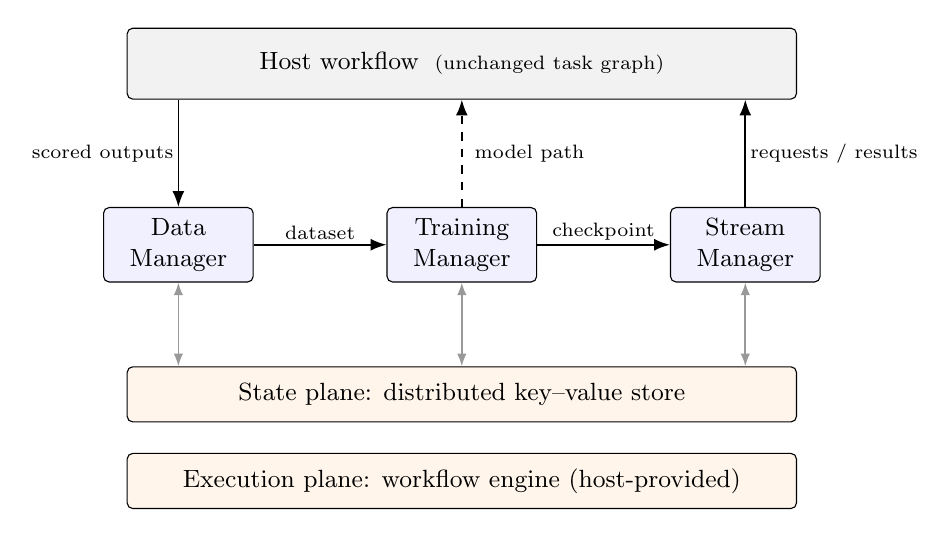
\begin{tikzpicture}[
      font=\small,
      node distance=0pt,
      box/.style={draw, rounded corners=2pt, align=center, inner sep=4pt},
      comp/.style={box, fill=blue!6, minimum width=19mm, minimum height=9mm},
      host/.style={box, fill=black!5, minimum width=85mm, minimum height=9mm},
      plane/.style={box, fill=orange!8, minimum width=85mm, minimum height=7mm},
      flow/.style={-{Latex[length=2mm]}, semithick},
      dashflow/.style={-{Latex[length=2mm]}, semithick, dashed},
      link/.style={{Latex[length=1.6mm]}-{Latex[length=1.6mm]}, semithick,
                   black!40},
      lbl/.style={font=\scriptsize, inner sep=1.5pt},
    ]
    % --- three components, evenly spaced on one row -----------------------
    \node[comp] (data)   at (-3.6, 0) {Data\\Manager};
    \node[comp] (train)  at ( 0.0, 0) {Training\\Manager};
    \node[comp] (stream) at ( 3.6, 0) {Stream\\Manager};

    % --- host workflow above, planes below --------------------------------
    \node[host]  (wf)    at (0,  2.3) {Host workflow \;{\scriptsize(unchanged
                                       task graph)}};
    \node[plane] (state) at (0, -1.9) {State plane: distributed key--value
                                       store};
    \node[plane] (exec)  at (0, -3.0) {Execution plane: workflow engine
                                       (host-provided)};

    % --- workflow <-> components ------------------------------------------
    \draw[flow] (wf.south -| data)   -- node[lbl, left]  {scored outputs}
                (data.north);
    \draw[flow] (stream.north)       -- node[lbl, right] {requests / results}
                (wf.south -| stream);
    \draw[dashflow] (train.north)    -- node[lbl, right=1mm] {model path}
                (wf.south);

    % --- component -> component (the only inter-component edges) ----------
    \draw[flow] (data.east)  -- node[lbl, above] {dataset}    (train.west);
    \draw[flow] (train.east) -- node[lbl, above] {checkpoint} (stream.west);
    % Both components also drive the execution plane; drawn as plain stubs
    % below rather than as edges, since neither addresses the other.

    % --- everything sits on the two shared planes -------------------------
    \draw[link] (data.south)   -- (state.north -| data);
    \draw[link] (train.south)  -- (state.north);
    \draw[link] (stream.south) -- (state.north -| stream);
  \end{tikzpicture}
  \caption{ROME-A architecture. The three components interact only through the
  state plane; both they and the host workflow's own tasks are executed by a
  single, host-provided workflow engine. The dashed edge is the optional path by
  which a workflow that owns its own inference collects improved weights.}
  \label{fig:architecture}
\end{figure}

\subsection{Data Manager}
\label{sec:design:data}

The data manager converts the by-products of a running campaign into a training
corpus. Its contract with the workflow is a single call, made from wherever a
scored artifact happens to be produced:

\begin{lstlisting}[style=rome]
rome.add_training_data(prompt=p, completion=c, score=r)
rome.add_training_data(sequence=s, pdb_path=f, score=plddt, pTM=t, pAE=e)
\end{lstlisting}

Records are untyped keyword payloads. This is the concession that buys R2: the
data manager attaches provenance (a unique identifier, an arrival timestamp, and
the model version in force at the time) and otherwise treats a record as opaque.
Interpretation is deferred to the training task, which is the only component
that must understand the modality.

\paragraph{Admission and egress policy.}
A campaign generates far more artifacts than are worth training on, and the
criterion for ``worth training on'' is domain knowledge the framework does not
have. The data manager therefore exposes policy as configuration rather than
code: an admission predicate applied on ingress, an optional deduplication key,
and a sampling strategy applied on egress. IMPRESS-R supplies as its admission
predicate exactly the confidence thresholds the campaign already uses to decide
that a design is worth keeping, so the corpus is the campaign's own accepted
designs and no separate quality model is introduced.

Filtering on ingress and sampling on egress is a deliberate split. Ingress
filtering is a statement about validity---a design below threshold is not
evidence---and is therefore permanent. Sampling is a statement about what this
particular round should learn from, and must be revisited each round; making it
an egress-time function lets a strategy such as ``the $k$ highest-scoring
designs so far'' see designs that were added before the previous round ran.

\paragraph{Monotonicity and the training watermark.}
The corpus is monotone: records are added and never invalidated by subsequent
model versions. A record produced under version~1 remains valid training
evidence after version~2 is published; the version stamp is provenance, not an
expiry. What advances instead is a \emph{consumption watermark}. Writing $|C|$
for the corpus size and $c$ for the watermark, the manager reports
$u = |C| - c$ unconsumed records, and a training round is possible when
$u \geq \tau$ for a configured threshold~$\tau$. A completed round sets
$c \leftarrow |C|$. Two properties follow that a purely size-based trigger does
not give: rounds after the first are driven by \emph{new} evidence rather than
by the accumulated corpus re-crossing a threshold, and a round may still train
on the full corpus if its sampling strategy asks for it, because consumption
does not delete.

\subsection{Stream Manager}
\label{sec:design:stream}

Inference and reward evaluation are not one-shot calls in a self-improving
campaign; they are demanded continuously for its whole duration, and the cost of
initializing them---loading a multi-billion-parameter model onto a GPU---is
large relative to a single request. The stream manager therefore runs them as
\emph{persistent} tasks, submitted to the workflow engine as long-lived services
that hold their model resident and consume requests until the campaign ends.

A stream group is a set of identical replicas sharing a configuration. Requests
submitted to a group are distributed across its replicas, and results are
collected by group, so scaling inference throughput is a change to one integer
rather than a change to the workflow's structure.

\paragraph{Inversion of control.}
The inference and reward code belongs to the workflow. ROME-A supplies the loop
around it and, by default, requires only a per-batch function
$f: \text{inputs} \rightarrow \text{results}$ and an optional loader
$g: \text{path} \rightarrow \text{model}$. Neither signature is ROME-specific,
so existing code is usually reusable verbatim; a context handle exposing the
loaded model, the stop and reload signals, and the shared store is passed only
to functions whose signature has a place for it. A workflow with an
irreducibly custom loop---one that batches adaptively, or interleaves its own
bookkeeping---may instead supply the loop body itself and receive the same
context, retaining ROME-A's weight synchronization while owning its own
scheduling.

\paragraph{Fault containment.}
A stream is a shared resource: a reward stream serves every backbone in a
campaign. Propagating a failure from one request to the task would take down
work unrelated to the malformed input that caused it. Failures are therefore
scoped to the request---the error is recorded as that request's result and the
loop continues---so that a single unparseable payload cannot cost the campaign
a GPU-resident model.

\subsection{Training Manager}
\label{sec:design:training}

The training manager answers three questions and performs one action. The
questions are whether training is currently \emph{possible}, whether it is
\emph{running}, and whether it is \emph{finished}; the action is to run a round
and publish its result. Distinguishing ``not possible yet'' from ``possible''
matters to a host workflow that wants to decide, for example, whether to
continue a campaign or to wait for an improved model before starting the next
cycle---a distinction a boolean \texttt{is\_training} flag cannot express.

Rounds are triggered in either of two ways. Automatically, a poll loop in the
manager process observes the data manager's watermark and starts a round when
$u \geq \tau$; the campaign then improves its model without any explicit
orchestration in the workflow. Manually, the workflow calls
\texttt{start\_training()} directly, which is appropriate when the natural
trigger is a phase boundary in the science rather than a data volume.

Only the round itself is submitted to the execution plane. The poll loop is
cheap and runs in the manager's own process; the training task carries the
resource requirements declared by the training algorithm and is placed by the
engine like any other task.

\paragraph{Checkpoint publication.}
A completed round writes a checkpoint and makes it visible through two keys in
the state plane: a path~$p$ and a monotonically increasing version~$v$. The
publication order is load-bearing. The manager writes~$p$ and only then
increments~$v$; every reader gates on~$v$ and, upon observing an increase, reads
whatever~$p$ currently holds. Since single-key writes are atomic and $v$ is
incremented by exactly one writer, a reader that observes $v' > v_i$ (its local
version) always reads a path belonging to some version $\geq v'$. It may skip an
intermediate version if rounds complete faster than it polls, but it can never
read a path that is stale relative to the version that prompted the read, and it
can never observe a version whose path has not yet been written. The protocol
therefore needs no lock, no barrier, and no acknowledgment from readers.

\begin{algorithm}[t]
\caption{Checkpoint publication and weight synchronization. Top: the training
manager, the single writer of $(p, v)$. Bottom: the loop of one stream replica
$i$, with local version $v_i$. The two run concurrently on different nodes and
synchronize only through $(p, v)$.}
\label{alg:publish}
\begin{algorithmic}[1]
\Statex \textbf{Training manager (writer)}
\State $D \gets \Call{Sample}{C}$ \Comment{egress policy over the corpus}
\State $p' \gets \Call{Train}{D}$ \Comment{submitted to the execution plane}
\State $p \gets p'$ \Comment{path written first}
\State $v \gets v + 1$ \Comment{then version; readers gate on this}
\State $c \gets |C|$ \Comment{advance the consumption watermark}
\State \Call{Notify}{$p', v$} \Comment{fan out to registered listeners}
\Statex
\Statex \textbf{Stream replica $i$ (reader)}
\While{$\neg$\Call{Stopped}{}}
  \If{$v > v_i$} \Comment{checked \emph{between} batches only}
    \State $M_i \gets \Call{Load}{p}$
    \State $v_i \gets v$
  \EndIf
  \State $B \gets \Call{Claim}{Q_i, b}$ \Comment{claim by removal; see \S\ref{sec:design:state}}
  \State \Call{Emit}{$f(B, M_i)$}
\EndWhile
\end{algorithmic}
\end{algorithm}

\paragraph{Reload granularity.}
A replica tests for a new version between batches, never within one
(Alg.~\ref{alg:publish}, line~8). An in-flight request is thus never interrupted,
and the visible cost of a model swap is bounded by one batch of latency rather
than by a cancellation and retry. When the training algorithm produces a
low-rank adapter rather than full weights, the swap itself is an adapter-sized
read against a resident base model, which is what makes mid-campaign weight
updates affordable at all.

\subsection{Composition: closing the loop}
\label{sec:design:loop}

The three components are independent, and one connection makes them a
self-improvement system: the training manager's checkpoint notification
(Alg.~\ref{alg:publish}, line~6) is registered as the stream manager's reload
trigger. A completed training round \emph{is} the event that moves inference
onto the new model. No component polls another, no component holds a reference
to another, and the host workflow does not sequence the handover.

Symmetrically, a reward stream's outputs are routed into the data manager, so
that scoring a candidate and contributing it as training evidence are the same
act. Both connections are established by the composing manager at startup and
both are configuration: a workflow that wants to decide for itself when
inference switches models disables the first, and a workflow whose reward stream
produces something other than training records overrides the second.

\subsection{State plane and concurrency}
\label{sec:design:state}

R3---concurrent contribution from tasks on many nodes without loss---is the
constraint that fixes the layout of ROME-A's shared state. The natural encoding,
a single key holding the corpus, is unsafe: read--modify--write of a shared
container drops records whenever two nodes interleave, and no ordering of the
operations avoids it without a distributed lock on the critical path of every
contribution.

ROME-A instead stores every record, request, and result under its own key and
reconstructs collections by scanning a key prefix. Single-key writes are atomic
in the underlying store, so concurrent producers cannot clobber one another and
no lock is required. Collection membership is a property of the key space rather
than of any one value, which also makes the layout tolerant of a producer
failing between operations: a partially-written collection is not a possible
state.

The same layout yields exactly-once request handling. A stream replica claims
work by \emph{removing} a request key: the removal succeeds for one claimant and
fails for every other, so a request is processed by exactly one replica without a
claim protocol, a lease, or a coordinator. Results are written under the request
identifier, so a caller can either await one specific request or drain the
group's completed results in bulk.

Counters that are not amenable to this treatment---the model version, the
consumption watermark---are each written by exactly one component, and are
therefore free of the read--modify--write hazard by construction rather than by
enforcement. Table~\ref{tab:state} summarizes the ownership discipline.

\begin{table}[t]
  \centering
  \small
  \caption{State-plane ownership. Every mutable datum has exactly one writer, so
  no cross-node lock appears on any contribution path.}
  \label{tab:state}
  \begin{tabular}{@{}lll@{}}
    \toprule
    Datum & Writer & Readers \\
    \midrule
    Corpus records      & any workflow task & Training Manager \\
    Consumption watermark & Training Manager & Training Manager \\
    Checkpoint path $p$   & Training Manager & streams, workflow \\
    Model version $v$     & Training Manager & streams, workflow \\
    Stream requests       & any workflow task & one stream replica \\
    Stream results        & one stream replica & workflow \\
    Stream status         & owning replica    & Stream Manager \\
    \bottomrule
  \end{tabular}
\end{table}

Finally, ROME-A namespaces all of its keys under a reserved prefix, so a host
workflow may pass in the store it is already using rather than provisioning a
second one, and the two sets of keys cannot collide.

\subsection{Extensibility}
\label{sec:design:extensibility}

R4 requires that a new model or training algorithm be a task, not a framework
modification. ROME-A's training interface is accordingly one method:

\begin{lstlisting}[style=rome]
class MyTrainer(rome.TrainTask):
    def train(self, dataset, output_dir, **kwargs) -> str:
        ...                  # dataset: whatever the Data Manager built
        return output_dir    # path the streams will reload from
\end{lstlisting}

The implementation receives the dataset and a destination and returns a
checkpoint path. Everything else---when the round fires, which records it sees,
where it is placed, who is notified of the result---is supplied by the training
manager and is not reimplemented. Resource requirements are declared as
attributes of the task rather than as arguments at a call site, so the same
declaration is used every round and the scheduling metadata travels with the
algorithm that needs it.

Two trainers accompany ROME-A and exercise opposite ends of the design space:
GRPO over a transformer language model, which consumes a tabular dataset,
requires a GPU per rank, and emits a low-rank adapter; and ProteinMPNN
fine-tuning for IMPRESS-R, which consumes structure--sequence records, writes an
on-disk shard for an external trainer, and emits full weights. Neither appears
in the data, stream, or training managers, and the framework contains no branch
on which of them is in use.

\subsection{Adoption cost}
\label{sec:design:adoption}

The design goal of \S\ref{sec:design:requirements} reduces, for a workflow that
already exists, to the following. Listing~\ref{lst:adoption} is the complete
integration for a campaign that keeps its own inference: a constructor
expressing policy, one call in the inner loop to contribute evidence, one call
to collect improved weights, and teardown.

\begin{lstlisting}[style=rome, caption={Complete ROME-A integration for a
workflow that owns its own inference. The campaign's task graph is
unchanged.}, label={lst:adoption}]
manager = rome.Manager(
    asyncflow,                              # the workflow's own engine
    data_config=rome.DataConfig(
        min_samples=64,
        filter_func=confidence_threshold),  # domain policy
    trainer_config=rome.TrainerConfig(
        trainer=ProteinMPNNTrainer()))
await manager.start()

for cycle in campaign:                      # unchanged
    weights = manager.get_current_model()   # None before the first round
    designs = run_cycle(cycle, weights)
    for d in designs:
        manager.add_training_data(**d)

await manager.stop()
\end{lstlisting}

Nothing in the loop is conditioned on ROME-A's internal state: before the first
round completes, \texttt{get\_current\_model()} returns nothing and the campaign
runs exactly as it did without ROME-A. Self-improvement is therefore additive to
an existing workflow in the strict sense---it changes what the campaign
converges to, not how the campaign is written.


\begin{thebibliography}{9}
\bibitem{dragon} Dragon: a distributed run-time for HPC and AI workflows.
\bibitem{asyncflow} RADICAL AsyncFlow: asynchronous workflow execution.
\end{thebibliography}

\end{document}
